
Este trabajo ha sido realizado por \theauthor y está dirigido a 1 de Bachillerato del itinerario de Ciencias Sociales.
%
No trata una unidad didáctica específica, sino que se enfoca a la presentación de la asignatura el primer día de clase.


\section{Introducción}


\subsection{Elección y Justificación}

Matemáticas es una asignatura que a bastante porcentaje del alumnado se le hace difícil. 
%
Hay algunos que optan por otros itinerarios sólo para evitar las Matemáticas, porque ya les parecen imposibles.
%
Hay otros que eligen Matemáticas "fáciles" (Matemáticas aplicadas a las Ciencias Sociales) porque no quieren ni Física ni Latín.

Sin saber con seguridad qué porcentaje del alumnado de esas "Matemáticas fáciles" la ha escogido por gusto o por ser la opción \textit{menos mala}, creemos que a un alto porcentaje del alumnado de 1 de Bachillerato de Sociales no le gustan las Matemáticas y que, además, pueden pensar que se les da realmente mal. 
%
Es por ello que queríamos hacer el trabajo para, de alguna manera, solucionar este problema que creemos que se da en el Bachillerato de Sociales.

Aunque una consigna de este trabajo era explicar un contenido didáctico de algún curso, habiendo pedido permiso, le hemos dado otro enfoque. 
%
Queríamos preparar la primera clase del curso de Matemáticas aplicadas a las Ciencias Sociales y queríamos hacerlo para motivarles y ayudarles a automotivarse.

A continuación, procedemos a definir más concretamente los objetivos.


\subsection{Objetivos}

\paragraph{Objetivo general}
\begin{itemize}
	\item Motivar al alumnado de Matemáticas aplicadas a las CC.SS.\footnote{Asignatura impartida en primero de Bachillerato.} para intentar romper la preconcepción negativa que puedan tener sobre las Matemáticas. 
\end{itemize}

\paragraph{Objetivos específicos}
\begin{itemize}
	\item Explicar el concepto de la Indefensión Aprendida\footnote{Definida en \ref{defn::indefension}.}. Puede ser que algún alumno haya \textit{aprendido la indefensión} hacia las Matemáticas. El primer paso para romper esa indefensión es conocer que existe y que es aprendida.
	\item Introducir el curso de Matemáticas y motivar a los alumnos.
	\subitem Hacer hincapié en que estas no son las Matemáticas fáciles, sino las útiles. Esto puede contribuir a que no se sientan "más tontos" (en las Matemáticas) que sus sus compañeros de las Matemáticas Académicas, ya que sus Matemáticas (CCSS) no son más fáciles, sino que tienen otro objetivo y son más aplicables.
	\item Mostrar el potencial de las Matemáticas aplicadas a las Ciencias Sociales para hacer más fuerte la motivación de los alumnos hacia la asignatura y complementar el objetivo anterior.
	\subitem En esta muestra, introducir algún recurso educativo como el material manipulativo.
\end{itemize}


\subsection{Contenidos}

No es necesario \textbf{ningún conocimiento previo} por parte de los alumnos para seguir con facilidad esta presentación de la asignatura.

Los contenidos a tratar no son relativos a las matemáticas. 
%
Los únicos contenidos como tal que tratamos en este trabajo son la indefensión aprendida y la aplicación del método de Montecarlo.

\section{Desarrollo}

Hemos estructurado el trabajo en torno a los objetivos específicos. 
%
Primero, tratamos la indefensión aprendida y lo haremos mediante un experimento, para que lo vean de primera mano.
%
Una vez interiorizado el concepto de indefensión aprendida, procederemos a introducir brevemente algunos aspectos del curso, recalcando la importancia de la automotivación.
%
Esta introducción se basará en material audiovisual para captar mejor la atención de los alumnos.
%
Por último, realizaremos un cálculo del número π por el método de Montecarlo. 
%
Este método se basa fundamentalmente en la Estadística y en la Probabilidad, temario específico de Matemáticas Aplicadas a las Ciencias Sociales.
%
Este cálculo se realizará en 2 partes. Una primera de cálculo manual, con material manipulativo (granos de arroz) y una segunda parte de cálculo simulado por ordenador.
%
El cálculo por ordenador es fundamental para que los alumnos puedan ver que realmente se obtiene el número π (ya que el método manual tiene algunos problemas, que trataremos en \ref{pimanual})

\subsection{Indefensión Aprendida}
\label{defn::indefension}

Por motivos de claridad de este escrito, exponemos primero el concepto y después el experimento, aunque después, en la exposición, conviene realizar primero el experimento y después explicar el concepto.

\subsubsection{Concepto}

Lo primero de todo es definir el fenómeno:

\begin{defn}[Indefensión Aprendida]
Condición de un ser humano o animal que ha aprendido a comportarse pasivamente, con la sensación subjetiva de no poder hacer nada y que no responde a pesar de que existen oportunidades reales de cambiar la situación aversiva, evitando las circunstancias desagradables o mediante la obtención de recompensas positivas.
\end{defn}

Creemos que este fenómeno se da en las Matemáticas de la siguiente manera:
%
Existe una creencia generalizada de que las Matemáticas son difíciles y que por mucho que uno esfuerce, este pensamiento permea y le lleva a comportarse pasivamente, motivado por la sensación de no poder hacer nada.
%
Otra posibilidad (un ejemplo más claro y fuerte de la indefensión) es: si yo he estudiado con mucho esfuerzo Matemáticas y no la he conseguido aprobar, aprenderé que no puedo sacar las Matemáticas.
%
Hay personas a las que les puede pasar esto porque realmente su inteligencia Logico-Matemática no sea muy alta, pero creemos que hay muchos que, con una inteligencia Logico-Matemática más que suficiente, se estrellan con las Matemáticas, ¿por qué? 
%
Porque a lo largo de su vida de estudiante, pueden haber aprendido la indefensión hacia las Matemáticas. 
%
Y esta indefensión se puede haber aprendido porque un año (o más) han tenido profesores más exigentes o que no han sabido transmitir los conocimientos y además en casa han recibido comentarios del tipo "Pues será que no vales para las Matemáticas".
%
Estos 2 factores creemos que son muy frecuentes que se den juntos o separados y que induzcan a los estudiantes una indefensión que, por supuesto, se puede desaprender. Y para desaprenderla, el primer paso es conocer que existe.


\subsubsection{Experimento}

Para tratar el concepto, realizamos un experimento en el que induzcamos una pequeña indefensión a una parte del alumnado para evidenciar lo real que es este fenómeno.

Se dividirá a la clase en 2 grupos sin que ellos lo sepan.
%
Las llamaremos la mitad \textit{control} y la mitad \textit{experimental}.

Desde su perspectiva, la actividad a realizar será, dada una palabra, formar otra palabra en singular con las mismas letras.
%
Por ejemplo: dada la palabra \textit{\textsc{roma}} tendrán que escribir la palabra \textit{\textsc{amor}}. 
%
Cuando lo hayan conseguido, levantarán la mano y esperarán a que se pueda empezar la siguiente ronda.

El papel que juegan las 2 mitades es que no todos los alumnos van a recibir la misma palabra con la que trabajar. 
%
La mitad \textit{control} recibirá siempre palabras con las que se pueda hacer otra palabra, mientras que la mitad \textit{experimental} recibirá palabras con las que sea imposible escribir otra palabra con esas letras.

El desarrollo del experimento es el siguiente:

\begin{itemize}
	\item[0.-] Cada alumno tiene en su mesa 3 sobres de colores: uno rojo, otro amarillo y otro verde.
	\subitem Hay 2 tipos de sobres: los del grupo control y los del grupo experimental que habrán sido previamente diferenciados. En la figure \ref{imgclase} se puede apreciar cómo se preparó el experimento en la exposición.
	\item[1.-] Cuando el profesor diga, abrirán el primer sobre, extraerán el papel con la palabra escrita y tendrán que escribir una nueva palabra con las mismas letras. Cuando lo consigan, les pediremos que levanten la mano y la mantengan levantada.
	\item[2.-] Una vez terminado el primer sobre (y haciendo ver a los que no lo han resuelto que hay muchos compañeros que sí), procederemos con el segundo sobre de la misma manera.
	\item[3.-] De la misma manera, procederemos al último sobre. 
	%
	En este último sobre, tanto el grupo control como el grupo experimental tienen exactamente la misma palabra. 
	%
	Es de esperar que los miembros del grupo control realicen con mayor rapidez el tercer sobre, mientras que los miembros del grupo experimental puedan incluso llegar a no ser capaces.
\end{itemize}


\begin{figure}[hbtp]
\centering
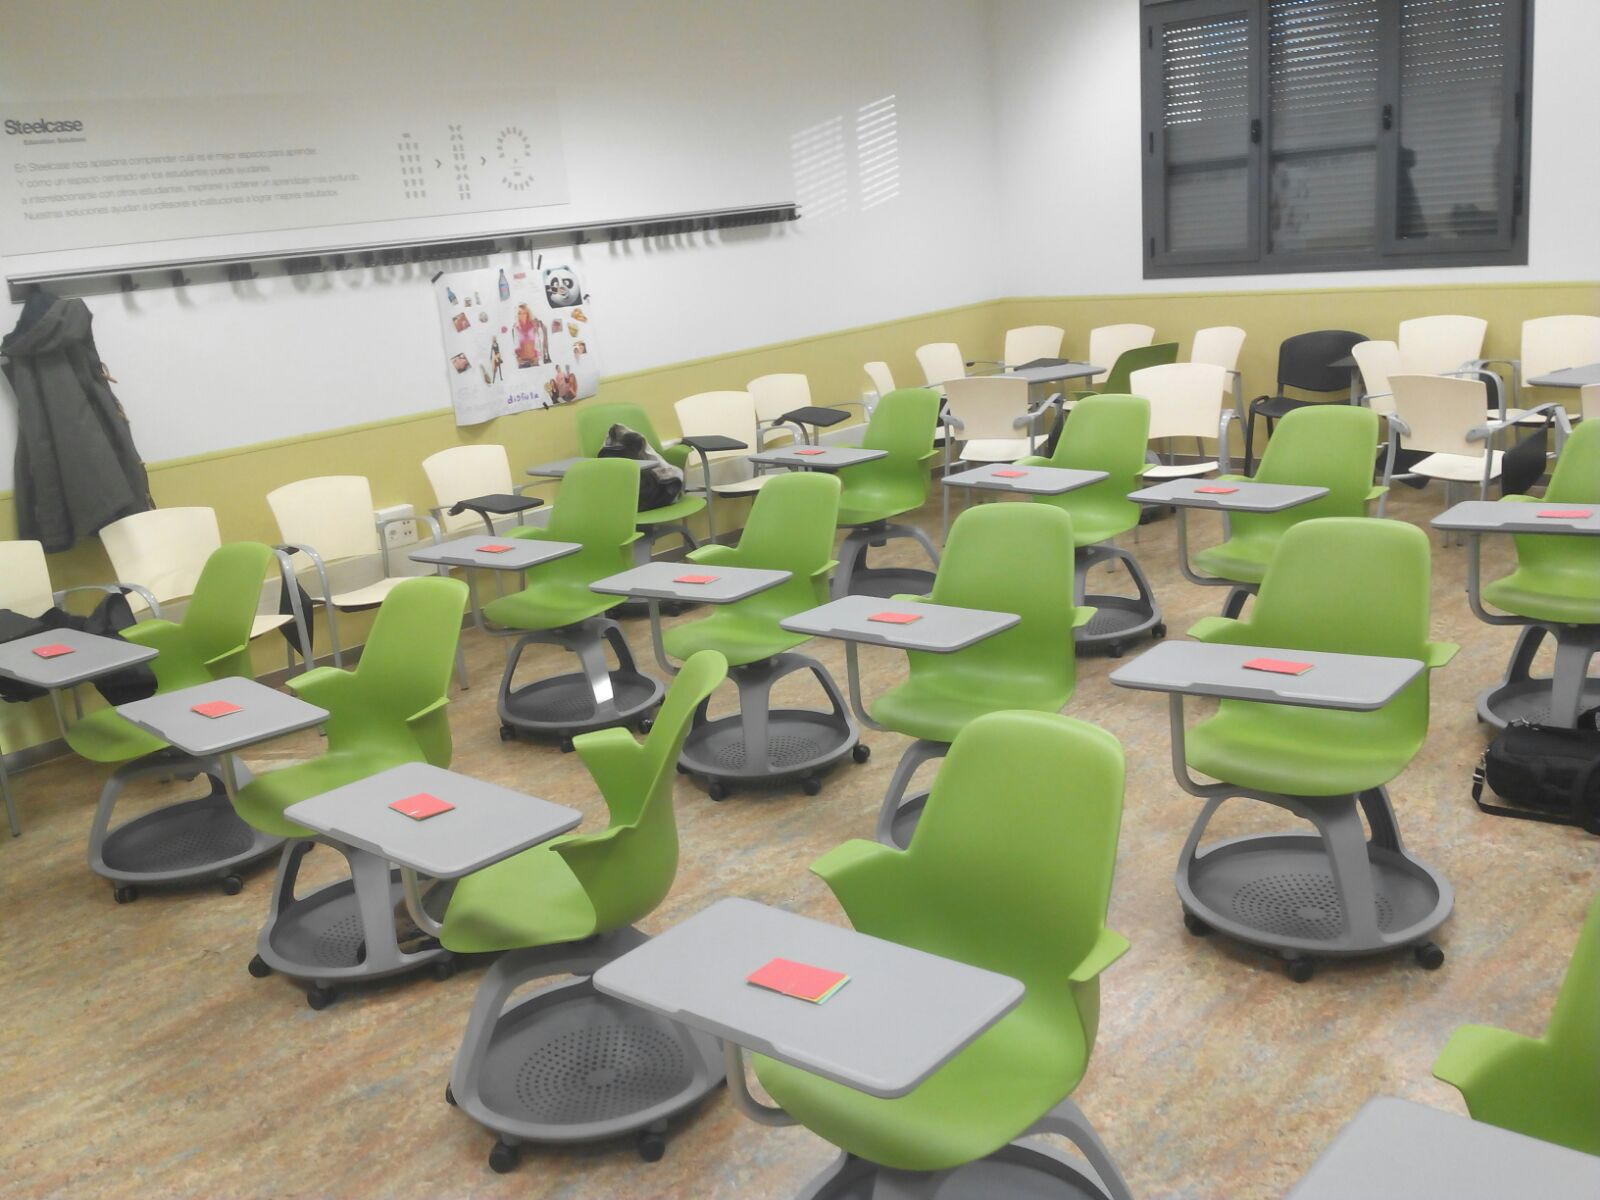
\includegraphics[scale=0.25]{img/clase.jpeg}
\caption{Clase con los sobres preparados, de tal manera que el grupo control está en la mitad izquierda y el experimental a la derecha.}
\label{imgclase}
\end{figure}


Una vez desarrollado el experimento, tendremos un rato de comentar la experiencia. 
%
Pediremos perdón por la pequeña "manipulación", ya que no todos tenían las mismas palabras y preguntaremos al grupo experimental cómo se han sentido.

\paragraph{Resultado en clase:} Muchos de los miembros del grupo \textit{experimental} manifestaban que se habían sentido impotentes e inútiles, llevándoles a no ser capaces de concentrarse para el último sobre.

Como decíamos anteriormente, una vez terminado el experimento en clase, procedemos a explicar el concepto, cómo se detecta y damos algunas herramientas para ponerle solución. 
%
Para más información sobre estos puntos, consultar la presentación de la exposición.

%{\LARGE \textcolor{red}{¿Incluir más descripción?}}

\subsection{Motivación}

Es en este punto de la clase donde arremetemos contra las ideas preconcebidas que puedan tener los alumnos sobre las Matemáticas y su relación con ellas. 
%
Lo ideal sería que empezaran el curso convencidos de que van a sacar las Matemáticas, igual que todas las demás, incluso, con buena nota.
%
Sin embargo, la realidad no suele ser la ideal y es probable que los alumnos hayan tenido problemas con las Matemáticas y crean, desde el primer día, que van a suspenderla.
%
Entablaremos un diálogo sobre su percepción de las Matemáticas, si creen que van a suspender y si se sienten identificados con la indefensión aprendida. Tal vez alguno detecta que le ha ocurrido.

Una vez finalizado, procederemos a dar una visión de las Matemáticas algo distinta a lo habitual: \textbf{las Matemáticas tratan de perspectivas}. 
%
Daremos varios ejemplos de cómo una misma situación tiene muchas perspectivas y como las Matemáticas llevan esto al extremo. 
%
Por poner un ejemplo, el número $\rfrac{4}{3}$ se puede representar de muchísimas maneras distintas, cambiando el sistema de representación, utilizando propiedades físicas, sonidos, etc. 
%
Algunos de estos ejemplos se encuentran en el vídeo de la presentación, obtenido de la charla de Roger Antonsen, \textit{Math is the hidden secret to understanding the world } (TED,2016).

Pondremos también ejemplos reales de perspectivas y de cómo jugar con estadísticas. 
%
En concreto, estos ejemplos versan sobre los datos de paro y resultados electorales publicados en medios de comunicación.
%
En las gráficas propuestas se observan incoherencias.


¿Qué relación tiene esto de perspectivas con estos alumnos? Son ellos quienes, en unos años, serán periodistas, economistas, incluso estadísticos y será su trabajo ser fiel a las representaciones de un mismo hecho e intentar aportar la mejor perspectiva posible. ¡Qué responsabilidad!

Por último, brevemente, indicaremos algunos de los problemas que se van a tratar en la asignatura a lo largo del año.
%
Estos son: optimización de los recursos para maximizar el beneficio (Optimización lineal), el concepto de normalidad y la predicción de variables que se distribuyen normalmente.

\subsection{Método Montecarlo para calcular π}
\label{pimanual}

Éste método se basa en la generación de números aleatorios para aproximar expresiones matemáticas complejas. 
%
El método se llamó así en referencia a la "capital del azar", el casino de Montecarlo.


Dividiremos a la clase por los grupos habituales de trabajo y les daremos a cada uno una cartulina cuadrada con pequeñas paredes y una circunferencia tangente a los lados del cuadrado pintada en el interior. Además, les entregaremos un puñado de arroz de unos 120 granos.
%
En la figura \ref{imgcartulinas} se puede ver el material preparado para ser entregado.

\begin{figure}[hbtp]
\centering
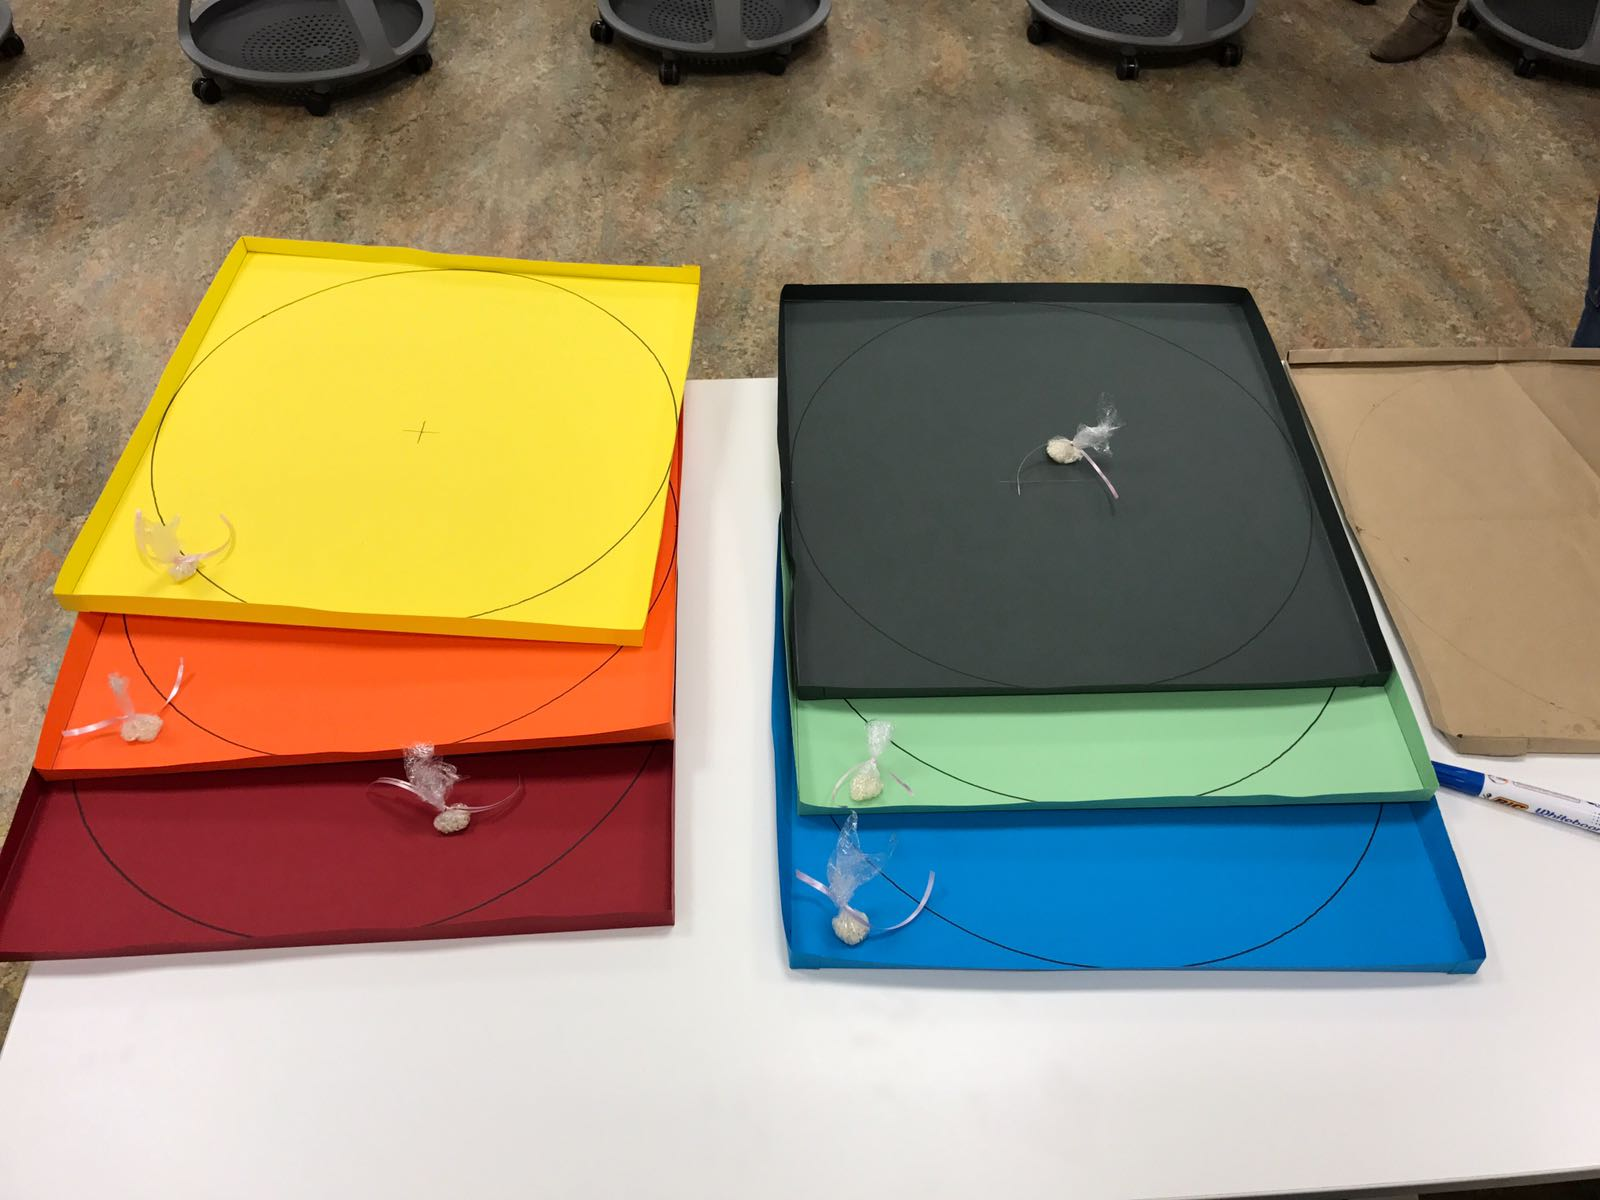
\includegraphics[scale=0.25]{img/cartulinas.jpeg}
\caption{Material preparado para ser entregado a cada grupo. 1 cartulina y una bolsita de arroz con 120 granos por equipo.}
\label{imgcartulinas}
\end{figure}

Un miembro del grupo lanzará el arroz sobre la cartulina y contarán el número de granos que han caído en el círculo y el número de granos que han caído en el cuadrado.
%
Sea $n_{cir}$ el número de granos en el círculo y $n_t$ el número de granos que han caído dentro del cuadrado (algunos de los cuales habrán caído dentro del círculo también).
%
Tendrán que realizar el cálculo $\rfrac{n_{cir}}{n_t}·4$.
%
El número que debería salir sería π. La demostración se encuentra en la figura \ref{imgpidemo}.

\begin{figure}[hbtp]
\centering
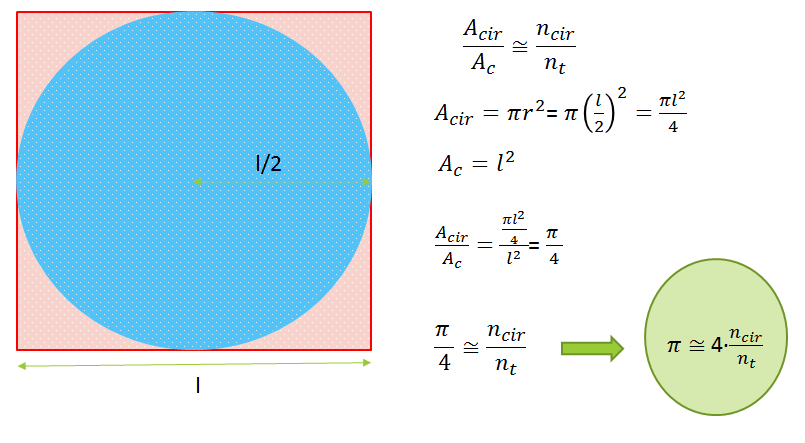
\includegraphics[scale=0.5]{img/pidemo.png}
\caption{Demostración de la relación entre la proporción de granos de arroz y el número π.}
\label{imgpidemo}
\end{figure}

\subsubsection{Limitaciones del experimento:}

Es probable que cada resultado obtenido no se acerque al número π. Esto se debe a algunos factores:

\label{ProblemasExperimento}
\begin{itemize}
	\item Los granos de arroz no se distribuyen uniformemente sobre la cartulina, es decir, no hemos generado puntos suficientemente aleatorios para realizar el experimento.
	\item El número de granos de arroz puede resultar insuficiente. Si cubriéramos absolutamente toda la superficie de la cartulina de granos de arroz, el cálculo sería mucho más exacto.
\end{itemize}

Debido a estos 2 factores, el método de Montecarlo consiste en realizar el experimento muchas veces y tomar la media y la distribución de los resultados obtenidos.

\paragraph{Resultado en clase:} Les propusimos hacer 4 lanzamientos por equipo y calcular la media de los resultados obtenidos. 
%
La mejor media fue $3.22$ y la peor fue $3.81$. 
%
Ninguno de los 2 resultados se acerca mucho, debido a los factores mencionados anteriormente.


\subsubsection{Simulación}

Por lo expuesto en \ref{ProblemasExperimento}, recurrimos a la tecnología, para realizar simulaciones.

Hemos programado un software en $R$ para realizar la simulación de tirar $n$ granos de arroz $m$ veces y estudiar la distribución.
%
Incluimos una imagen del histograma de uno de los resultados obtenidos utilizando $n=100$ y $m=10^5$ (Imagen \ref{imgpidist}). 

En la imagen se puede ver que alguno de los resultados obtenidos era cercano a $2.5$.
%
Es decir, el valor de π aproximado con 100 granos de arroz ha llegado a ser 2,5, una aproximación realmente mala.
%
Por este motivo es tan importante realizar la simulación muchas veces y estudiar la media y la distribución.
%
Se puede observar también que la distribución de los puntos es una distribución normal o gaussiana.

\begin{figure}[hbtp]
\centering
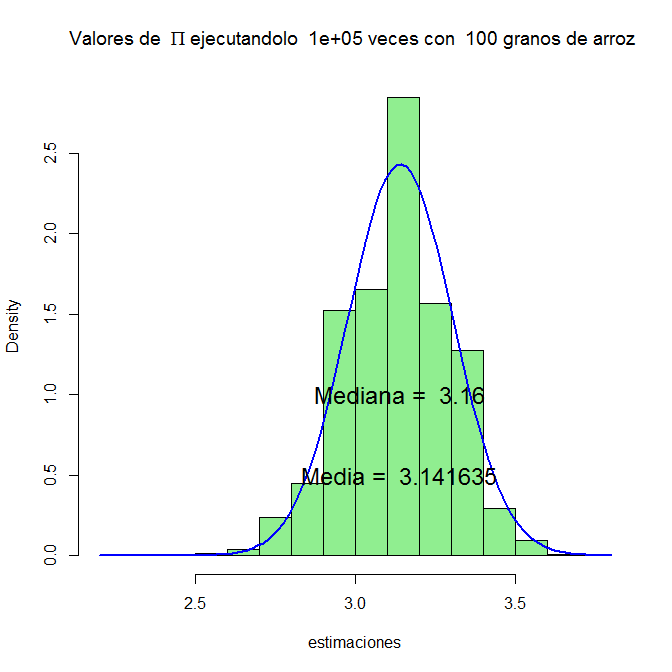
\includegraphics[scale=0.5]{img/piimagen.png}
\caption{Distribución de los valores obtenidos con $n=100$ y $m=10^5$.}
\label{imgpidist}
\end{figure}

\newpage
\section{Fuentes consultadas}

\begin{enumerate}
\item José María Sorando Muzás, \textit{Matemáticas en el debate Zapatero - Rajoy} (2008) [\url{http://catedu.es/matematicas_mundo/SOCIEDAD/sociedad_debate.htm}]
\item Josu Mezo, \textit{El peor gráfico para el peor resultado} (2015) [http://www.malaprensa.com/2015/06/el-peor-grafico-para-el-peor-resultado.html]
\item Will Smith, \textit{Pursuit of happiness} (2012).
\item Roger Antonsen, \textit{Math is the hidden secret to understanding the world } (TED,2016) [\url{https://www.youtube.com/watch?v=70WYy6qZHN4}]
\item Raúl Vaquerizo, \textit{Simulación. Estimación de pi con el método Montecarlo } [\url{http://analisisydecision.es/simulacion-estimacion-de-pi-con-el-metodo-montecarlo}]
\end{enumerate}

\section{Reflexión y autoevaluación}


\subsection{Autoevaluación}

Creemos que hay 2 aspectos fundamentales sobre los que autoevaluarnos. 
%
El primero, sobre el planteamiento del trabajo: el tema escogido, los objetivos y la idea para llevarlos a cabo.
%
El segundo, el desarrollo de la idea en la exposición en clase.

\subsubsection{Planteamiento}

Creemos que el tema elegido es un tema muy importante.
%
Hay muchos alumnos que se sienten indefensos ante las matemáticas, impotentes y así es muy difícil que puedan aprender Matemáticas y utilizarlas. Creemos que el primer paso es atajar esa negatividad.

Los objetivos específicos planteados creemos que están bien alineados con el objetivo general. 
%
Además, aportan una buena estructura para desarrollar la exposición.

Creemos que la manera en la que llevamos a cabo los objetivos fue adecuada, tocando muchos puntos distintos para captar la atención y animar a mantener la concentración: 
\begin{itemize}
	\item El experimento se desarrolla a base de un ejercicio sobre algo que, a priori, no tiene nada de matemáticas (podríamos decir que es un ejercicio rompedor)
	\item Utilización de recursos audiovisuales (presentacíón de PowerPoint, fragmentos audiovisuales)
	\item Utilización de las matemáticas en la vida real (Debate Rajoy-Zapatero).
	\item Material manipulativo.
	\item Nuevas tecnologías (simulación por ordenador).
\end{itemize}

Vemos muy positivo el amplio rango de recursos que se utilizan en este trabajo y además creemos que todos ellos tienen sentido, que no los utilizamos \textit{por utilizar}, sino que de verdad estaban bien enfocados y alineados con los objetivos.

Por comentar un aspecto del planteamiento que, tal vez, es mejorable sería la elección del experimento de montecarlo.
%
Tal vez si realizáramos el experimento de Montecarlo con otro fin distinto a aproximar el número π, los alumnos podrían disfrutarlo más.

Por mencionar un aspecto negativo, del que nos dimos cuenta gracias a las evaluaciones, es que la simuación del experimento de Montecarlo utilizando \textit{R} hace que pueda haber compañeros del máster que no quieran utilizar esta idea en su totalidad, ya que esa parte les resulta más complicada.
%
De todas formas, la simulación se puede realizar con otros programas que pueden estar más al alcance de cualquier docente.

\subsubsection{Desarrollo}

El desarrollo de la exposición se llevó a cabo satisfactoriamente.
%
Creemos que se cumplieron los objetivos:
\begin{itemize}
	\item \textbf{Indefensión aprendida:} hubo alumnos que confirmaron que se habían sentido impotentes y que, debido a los 2 fallos previos, ya no eran capaces de hacer la tercera.
	\item \textbf{Introducción del curso y Motivación:} las evaluaciones recibidas de nuestros compañeros eran positivas en cuanto a que supimos captar la atención de los supuestos alumnos y despertado interés sobre la asignatura.
	\item \textbf{Experimento de Montecarlo:} salió de los propios alumnos que el número que intentábamos aproximar era el número pi.
	%
	En las evaluaciones valoraban positivamente el experimento de Montecarlo, como dinámico y entretenido.
\end{itemize}

Por otro lado, en aspectos a mejorar: nos excedimos de los 40 minutos en el tiempo de la exposición. 
%
Aunque teníamos el planning y habíamos ensayado, en el momento del directo nos alargamos con los tiempos, provocando que el grupo siguiente al nuestro tuviera que hacer su exposición con cierta prisa.

\subsection{Reflexión}

Para la elección del tema se hizo una tormenta de ideas y luego decimos en conjunto cuál se elegía por lo que todos estuvimos de acuerdo y contentos con el tema expuesto.
%
Con la primera parte del trabajo queríamos motivar a los alumnos a que todos pueden hacer aquello que se proponen y quitarles esa indefensión aprendida a las matemáticas.
%
Con la segunda parte queríamos realizar algún tipo de juego de forma que aplicáramos unos de los recursos vistos en clase como son las matemáticas manipulativas.
%
Si bien es cierto, tuvimos dificultades con la elección del material para aplicar el método de Montecarlo ya que en principio la idea era hacer una diana en la pizarra y tirar tizas, pero comprobamos que eso no obtenía los resultados esperados.
%
Finalmente se optó por las cartulinas, aunque por la disposición de la clase sin mesas apropiadas donde apoyarlas también resultó algo peor de los que esperábamos.
%
No obstante, creemos que la idea quedo clara: \textit{motivación y utilidad de las matemáticas en el campo de las ciencias sociales}.

En general estamos bastante satisfechos con el resultado del trabajo, aunque los experimentos podrían haber salido mejor. 
%
El experimento de la indefensión aprendida no funcionó a la perfección, ya que hubo participantes que después de no haber conseguido las 2 primeras, sí consiguieron la última en un tiempo similar a los que habían conseguido las 2 primeras.
%
Sin embargo, el experimento evidenció el efecto que queríamos tratar, con lo que se cumplió el objetivo.
%
Además, nos hubiera gustado que los resultados del juego hubieran sido más próximos al número pi.




